%%%%%%%%%%%%%%%%%%%%%%%%%%%%%%%%%%%%%%%%%%%%%%%%%%%%%%%%%%%%%%%%%%%%%%%%%%%%%%
% RoboMaster EP Experiment 2 group report
% Layout adapted from Tau Class v2.6.0 by Guillermo Jimenez, CC BY 4.0.
% Official source: https://github.com/MemoJimenez/Tau-class
%%%%%%%%%%%%%%%%%%%%%%%%%%%%%%%%%%%%%%%%%%%%%%%%%%%%%%%%%%%%%%%%%%%%%%%%%%%%%%
\documentclass[9pt,a4paper,twocolumn,twoside]{tau-class/tau}
\usepackage[english]{babel}
\usepackage{tabularx}
\usepackage{tikz}
\usepackage{pgfplots}
\usetikzlibrary{arrows.meta,positioning}
\pgfplotsset{compat=1.18}
\graphicspath{{figures/}}

\definecolor{deepocean}{HTML}{17324D}
\definecolor{signalblue}{HTML}{1B6B8C}
\definecolor{softblue}{HTML}{EAF2F6}
\definecolor{resultgreen}{HTML}{287A57}
\colorlet{taucolor}{deepocean}
\hypersetup{
  pdftitle={RoboMaster EP Fixed-Point Grasping: Experiment 2 Group Report},
  pdfauthor={Yongyue Qi, Bo Ning, Junbiao Huang, Yutong Xue, Lintai Bao},
  pdfsubject={Robotics Integration Group Project I, Experiment 2}
}

\newcolumntype{Y}{>{\raggedright\arraybackslash}X}
\newcommand{\codepath}[1]{{\small\ttfamily\nolinkurl{#1}}}
\newcommand{\yes}{\textcolor{resultgreen}{\textbf{Yes}}}
\tikzset{
  task/.style={draw=signalblue,fill=softblue,rounded corners=2pt,
    minimum height=9mm,text width=21mm,align=center,font=\sffamily\scriptsize},
  taskarrow/.style={-{Latex[length=1.8mm]},thick,draw=signalblue}
}

\doctype{GROUP LABORATORY REPORT \textbullet\ EXPERIMENT 2}
\title{Fixed-Point Grasping with the DJI RoboMaster EP}

\author[1]{Yongyue Qi}
\author[1]{Bo Ning}
\author[1]{Junbiao Huang}
\author[1]{Yutong Xue}
\author[1]{Lintai Bao}
\affil[1]{Group E5 (S16--S20), Robotics Integration Group Project I}

\dates{Report date: 13 September 2026 \textbullet\ Platform: RoboMaster EP arm and gripper}
\docinfo{Student IDs: Yongyue Qi 24020036050; Bo Ning 24020036049;
Junbiao Huang 24020036027; Yutong Xue 24020036072; Lintai Bao
24020036004. Layout adapted from Tau Class v2.6.0 (CC BY 4.0).}
\footinfo{RoboMaster EP \textbullet\ Experiment 2}
\theday{13 September 2026}
\organization{Robotics Integration Group Project I}
\leadauthor{Group E5}

\begin{abstract}
This report documents a five-cycle fixed-point pick-and-place experiment using
the arm and gripper mounted on a DJI RoboMaster EP. A ROS 2 Humble and Gazebo
Fortress simulation produced five successful placements and five verified
returns home, with a mean horizontal error of 4.358 mm and a maximum of
5.604 mm. The group also observed five successful physical transfers without an
abnormal event. Hardware success is supported by the submitted video and team
observation; no instrumented hardware accuracy, force, payload, or timing data
are claimed. The report also states the interface differences introduced by
replacing the unavailable standalone mechArm 270 with the RoboMaster platform.
\end{abstract}
\keywords{fixed-point grasping, RoboMaster EP, ROS 2, Gazebo, pick-and-place,
repeatability}

\begin{document}
\maketitle
\thispagestyle{firststyle}

\section{Scope and Organization}

\subsection{Objective and platform adaptation}
\taustart{T}he required task is fixed-point pick-and-place without visual
localization: return home, approach point A, descend, grasp, lift, move to point
B, release, and return home. Acceptance requires at least four successful
transfers in five consecutive trials, together with collision, joint-limit, and
failure checks.

Because the specified standalone mechArm 270 was unavailable, the group used
the arm and gripper mounted on a DJI RoboMaster EP chassis. Simulation uses ROS
2 Humble, Gazebo Fortress, and custom kinematics/control. The physical test uses
the RoboMaster Python SDK. This is a documented platform adaptation, not proof
of an unchanged ROS 2 hardware backend.

\begin{info}
Simulation completed 5/5 placements and 5/5 verified returns home. The group
confirmed 5/5 physical transfers on 12 September 2026. Numerical accuracy is
available for simulation only; the physical result is observational.
\end{info}

\begin{table*}[t]
\caption{Team organization and principal responsibilities.}
\label{tab:roles}
\centering
\begin{tabularx}{0.96\textwidth}{@{}p{31mm}p{28mm}Y@{}}
\toprule
\textbf{Member} & \textbf{Area} & \textbf{Main responsibility}\\
\midrule
Bo Ning & Simulation & Environment, scene, models, resources, and launch setup.\\
Junbiao Huang & Simulation & Motion program, feedback logic, and repeated-cycle debugging.\\
Yongyue Qi & Analysis & Result/log audit, error analysis, report materials, and repository integration.\\
Yutong Xue & Hardware & Pick/release waypoints, approach/lift height, and gripper-retention checks.\\
Lintai Bao & Hardware & SDK communication, task sequence, chassis turn/return, and exception handling.\\
\bottomrule
\end{tabularx}
\tabletext{Xue and Bao jointly performed physical setup, parameter review, and integrated trials. All five members share the final project outcome.}
\end{table*}

\section{System Principle}

\subsection{Common task intent}
Both implementations follow the same functional sequence even though their
control interfaces and cycle boundaries differ.

\begin{figure*}[t]
\centering
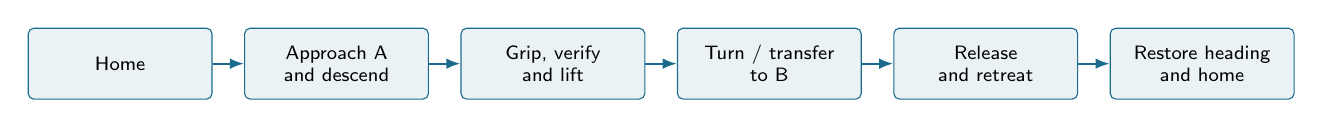
\begin{tikzpicture}[node distance=4mm]
\node[task] (home) {Home};
\node[task,right=of home] (approach) {Approach A\\and descend};
\node[task,right=of approach] (grip) {Grip, verify\\and lift};
\node[task,right=of grip] (transfer) {Turn / transfer\\to B};
\node[task,right=of transfer] (release) {Release\\and retreat};
\node[task,right=of release] (return) {Restore heading\\and home};
\draw[taskarrow] (home)--(approach);
\draw[taskarrow] (approach)--(grip);
\draw[taskarrow] (grip)--(transfer);
\draw[taskarrow] (transfer)--(release);
\draw[taskarrow] (release)--(return);
\end{tikzpicture}
\caption{Shared fixed-point grasping workflow.}
\label{fig:workflow}
\end{figure*}

\subsection{Simulation kinematics and feedback}
The simulated arm is represented by independent variables $r$ and $l$, with
linked joint coordinates
\begin{equation}
q_{\mathrm{arm1}}=r,\quad q_{\mathrm{arm2}}=l-r,\quad
q_{\mathrm{endpoint}}=-l,\quad q_{\mathrm{rod}}=l.
\end{equation}
The inverse calculation minimizes fingertip-centre error in the model's
$x$--$z$ plane. It rejects residuals above 0.002 m and solutions outside the
saved joint and coupling limits. Joint transitions use the quintic blend
$s(u)=10u^3-15u^4+6u^5$ to avoid discontinuous reference velocity.

Fresh bilateral gripper contact, retained-object height, and placement
conditions gate later phases. Placement requires horizontal error below 23 mm,
height error below 8 mm, and table contact. Home acceptance separately checks
heading, translation, and arm error over a stable interval.

\subsection{Physical workflow}
The final script initializes the RoboMaster in AP mode and commands the arm,
gripper, and chassis through the Python SDK. After each lift it stops the
chassis, clears previously buffered terminal input, and waits up to 30 s for a
fresh human confirmation that the object is retained. Only then is rotation
allowed. Odd cycles turn $+32^\circ$ from A to B; even cycles turn $-32^\circ$
from B to A. After cycle 5, the remaining heading is restored before the arm
moves through HIGH to HOME.

The confirmation is a supervised safety checkpoint, not a force or vision
measurement. Cleanup pauses the gripper, commands zero wheel speed, and closes
the SDK connection; it is not described as a certified emergency-stop system.

\section{Simulation Development}

\subsection{Scene and execution}
The scene contains a $1.6\,\mathrm{x}\,1.2\,\mathrm{x}\,0.05$ m table, a 25 mm cube, and fixed
points $A=(0.278,-0.001,0.0725)$ m and $B=(0.237,0.1453,0.0725)$ m. The cube's
simulation mass is 50 g; this is not a measurement of the real object. The
launch file starts Gazebo, the bridge, model spawning, state feedback, and the
task controller. Community model resources are attributed to
\href{https://github.com/jeguzzi/robomaster_ros}{jeguzzi/robomaster\_ros},
archived at commit \codepath{c05a39d7f0fa}.

\begin{figure}[H]
\centering
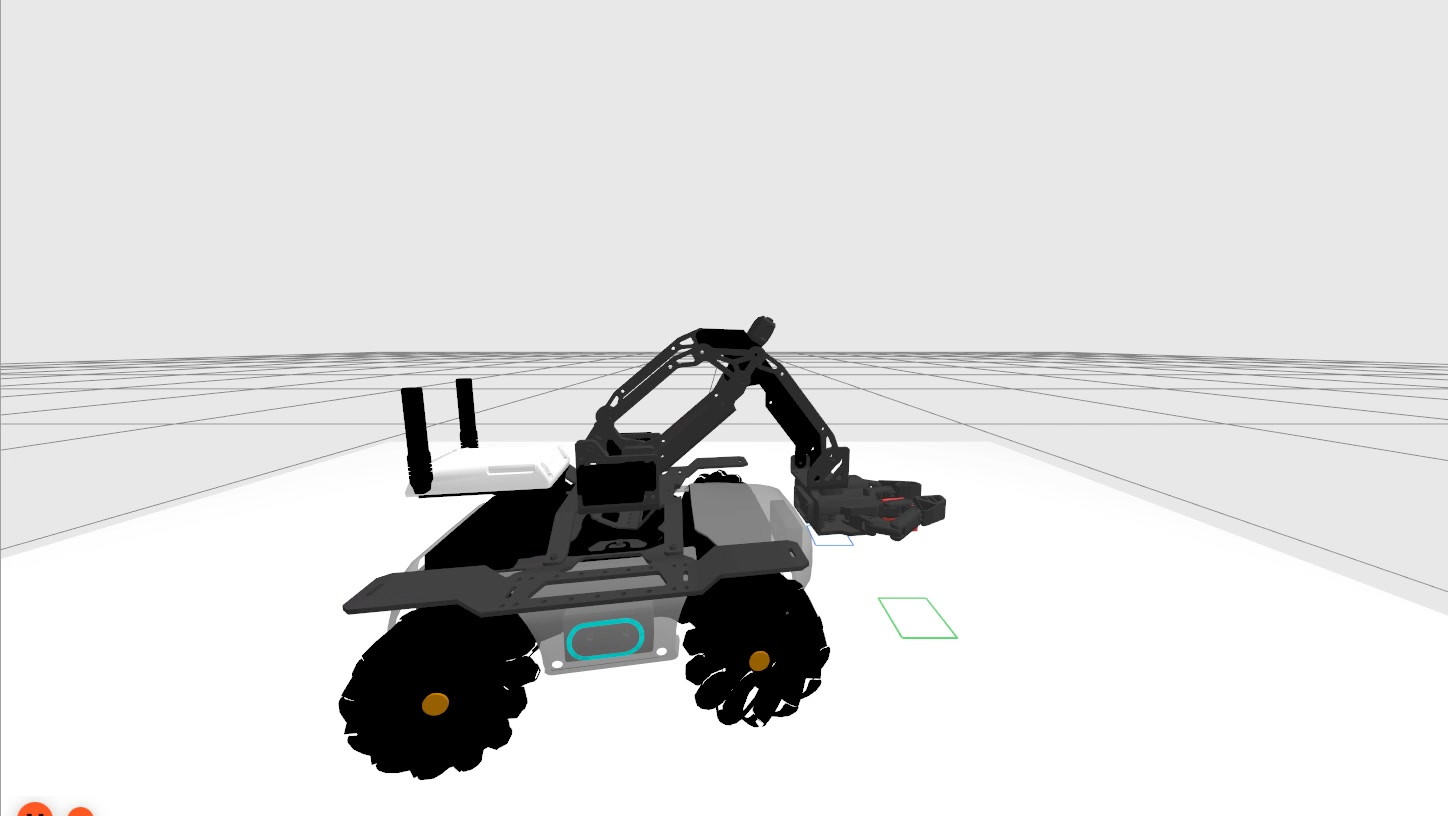
\includegraphics[width=0.94\columnwidth,trim=0 20 0 210,clip]{simulation_lift.jpg}
\caption{Recorded simulation frame during a lifted-object phase.}
\label{fig:sim}
\end{figure}

\subsection{Five-cycle result}
\begin{table}[H]
\caption{Main recorded simulation run.}
\label{tab:simresult}
\centering
\begin{tabular}{@{}crrrcc@{}}
\toprule
$n$ & \textbf{Err.} & \textbf{Head.} & \textbf{Time} & \textbf{Place} & \textbf{Home}\\
 & (mm) & ($^\circ$) & (s) & & \\
\midrule
1 & 2.274 & 0.445 & 67.01 & \yes & \yes\\
2 & 5.604 & 0.329 & 59.72 & \yes & \yes\\
3 & 4.192 & 0.404 & 60.92 & \yes & \yes\\
4 & 4.577 & 0.459 & 61.09 & \yes & \yes\\
5 & 5.144 & 0.405 & 61.29 & \yes & \yes\\
\bottomrule
\end{tabular}
\end{table}

Mean horizontal error was 4.358 mm and the maximum was 5.604 mm. The five cycle
intervals totalled 310.03 s; the run from initial home entry to final completion
lasted 318.02 s. The trajectory contains 4475 rows over a longer span because it
includes idle recording, so row span is not used as task time.

\begin{figure}[H]
\centering
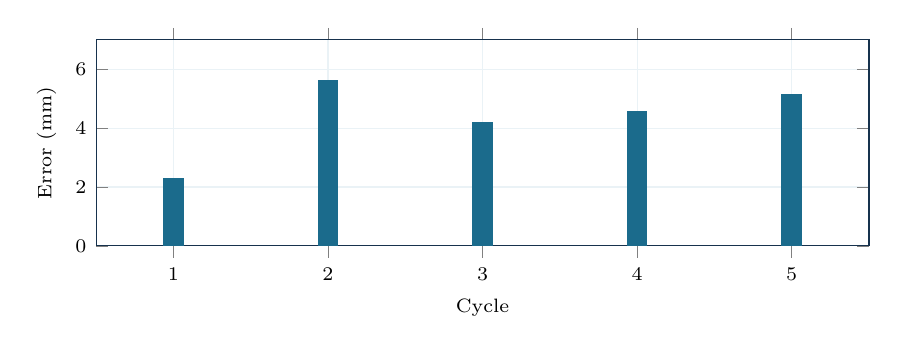
\begin{tikzpicture}
\begin{axis}[width=0.94\columnwidth,height=42mm,ybar,bar width=7pt,
  xlabel={Cycle},ylabel={Error (mm)},xmin=.5,xmax=5.5,ymin=0,ymax=7,
  xtick={1,2,3,4,5},grid=major,grid style={draw=softblue},
  axis line style={draw=deepocean},tick label style={font=\scriptsize},
  label style={font=\scriptsize}]
\addplot[fill=signalblue,draw=signalblue] coordinates
  {(1,2.274)(2,5.604)(3,4.192)(4,4.577)(5,5.144)};
\end{axis}
\end{tikzpicture}
\caption{Horizontal placement error by cycle.}
\label{fig:error}
\end{figure}

\section{Hardware Validation}

\subsection{Final physical parameters}
\begin{table}[H]
\caption{Arm waypoints used in the physical workflow.}
\label{tab:waypoints}
\centering
\begin{tabular}{@{}lrrl@{}}
\toprule
\textbf{Point} & $x$ & $y$ & \textbf{Function}\\
 & (mm) & (mm) & \\
\midrule
HOME & 82 & 80 & Retracted high\\
HIGH & 191 & 80 & Extended high\\
HOVER & 191 & $-1$ & Approach / lift\\
GRASP & 191 & $-51$ & Pick / release\\
\bottomrule
\end{tabular}
\end{table}

The arm descends from HOVER to GRASP, closes the gripper at SDK power 100, lifts
50 mm, and waits for human confirmation. The physical workflow alternates
A$\rightarrow$B and B$\rightarrow$A because it does not automatically replenish
the object. Simulation instead uses a refill node after home verification for
cycles 1--4 only.

\subsection{Observed outcome}
\begin{table}[H]
\caption{Team-observed physical transfers.}
\label{tab:hardware}
\centering
\begin{tabular}{@{}ccll@{}}
\toprule
$n$ & \textbf{Direction} & \textbf{Transfer} & \textbf{Abnormality}\\
\midrule
1 & A$\rightarrow$B & Successful & None observed\\
2 & B$\rightarrow$A & Successful & None observed\\
3 & A$\rightarrow$B & Successful & None observed\\
4 & B$\rightarrow$A & Successful & None observed\\
5 & A$\rightarrow$B & Successful & None observed\\
\bottomrule
\end{tabular}
\tabletext{All five lifts were confirmed. This is a team-observed record, not a sensor-generated hardware log.}
\end{table}

\subsection{Separate video evidence}
The real-device video is submitted as a separate artifact and is not embedded in
this PDF. Visual review confirms the RoboMaster EP arm, gripper, target cubes,
and operator terminal.

\begin{table}[H]
\caption{Hardware-video metadata.}
\label{tab:video}
\begin{tabularx}{\columnwidth}{@{}p{22mm}Y@{}}
\toprule
\textbf{Field} & \textbf{Recorded value}\\
\midrule
Filename & \codepath{RoboMaster_EP_Hardware_Demonstration.mp4}\\
Duration & 74.87 s\\
Frame & $1280\,\mathrm{x}\,720$ at 29.97 fps\\
Encoding & HEVC Main; AAC LC stereo\\
Size & 8,024,795 bytes\\
SHA-256 & \scriptsize\ttfamily 614a8eb55d8883cce4494496a199c828\\
& \scriptsize\ttfamily bb679b693f58a325319570a89fad6a6e\\
\bottomrule
\end{tabularx}
\end{table}

\section{Problems and Solutions}

\subsection{Resources and reference frames}
Early model problems included unresolved mesh paths and inconsistent
end-effector references. The archive bundles the model dependency and provides
\codepath{prepare_paths.py} to construct a runtime copy using local mesh paths.
Kinematics uses the forward ends of gripper link 4 rather than a rear linkage,
separating resource-resolution failures from control failures.

\subsection{Unstable lift and false closure}
A close command does not prove object retention. Simulation combines fresh
bilateral contact, a small closure preload, a hold interval, and an object-height
check. Hardware uses a 50 mm lift and fresh human confirmation. Neither proves
gripping force, but both prevent command completion from being misclassified as
a successful grasp.

\subsection{Repeated-cycle state}
Earlier sequences could drift or stop after one cycle. The final simulation
records five placement checks, five home checks, and four refill acknowledgments,
then ends after cycle 5. Hardware alternates directions and compensates the
remaining heading after cycle 5.

\subsection{Abnormal-case evidence}
Archived notes record eight passing offline tests across model and five-cycle
checks. An unreachable target such as $(10,10,0.6)$ is rejected by the solver
with a \codepath{ValueError}; joint and coupling limits are checked before
motion. Runtime stale-feedback and phase-timeout guards also exist. No separate
system-level fault-injection run or individual safety-check record was supplied.

\begin{table*}[t]
\caption{Requirements, deviations, and evidence status.}
\label{tab:limits}
\centering
\begin{tabularx}{0.96\textwidth}{@{}p{48mm}Y@{}}
\toprule
\textbf{Handout expectation} & \textbf{Evidence status}\\
\midrule
mechArm 270 hardware & Replaced by RoboMaster EP because of equipment availability.\\
Same ROS 2 interface for hardware & Not demonstrated; hardware uses the RoboMaster Python SDK.\\
Parameter-only migration & Not demonstrated across the different control backends.\\
Each member's individual safety check & No separate individual check record was supplied.\\
At least 4/5 transfers & Met in the recorded simulation and team-observed hardware outcome.\\
\bottomrule
\end{tabularx}
\end{table*}

\section{Repository Traceability}
The public shared repository is
\href{https://github.com/ccx8kg5qpd-debug/robomaster-ep-fixed-point-grasping}
{github.com/ccx8kg5qpd-debug/robomaster-ep-fixed-point-grasping}. The experiment
was completed before repository assembly. The history records the genuine
review, organization, publication, and reporting sequence on 13 September 2026;
it is not presented as a fabricated contemporaneous development history.

\begin{figure*}[t]
\centering

\includegraphics[width=0.70\textwidth]{commit_history_current.png}
\caption{Ten repository commits visible after video upload and before addition
of the first group-report build. Later commits added report materials.}
\label{fig:commits}
\end{figure*}

\section{Submission and Conclusion}

\subsection{Group package manifest}
\begin{table}[H]
\caption{Materials required by the handout.}
\label{tab:manifest}
\begin{tabularx}{\columnwidth}{@{}Yp{14mm}@{}}
\toprule
\textbf{Material and package location} & \textbf{Status}\\
\midrule
ROS 2 program, launch, and parameters: \codepath{01_simulation/} & Included\\
Model and point/height setup: \codepath{01_simulation/} & Included\\
Simulation video: \codepath{03_videos/simulation/} & Included\\
Real-device video: \codepath{03_videos/hardware/} & Included\\
Five-cycle records: \codepath{04_results/} & Included\\
Abnormal-test notes: \codepath{04_results/validation_record.md} & Limited\\
Brief group report: \codepath{05_group_report/} & Included\\
GitHub link and commit evidence: report and README & Included\\
\bottomrule
\end{tabularx}
\end{table}

\subsection{Reproducibility}
Simulation targets ROS 2 Humble and Gazebo Fortress on the team's Jetson Linux
environment. The startup wrapper contains a workspace path that must be adapted
on another machine. The model dependency is bundled with attribution. Saved
\codepath{results.json}, \codepath{events.jsonl}, and
\codepath{trajectory.csv} support independent checking of the numerical results
without rerunning Gazebo.

\subsection{Conclusion}
The evidence supports five successful simulation cycles with home verification
and five team-confirmed physical transfers without observed abnormality. The
project demonstrates a complete fixed-point sequence on the available RoboMaster
EP. Its strongest quantitative evidence is the saved simulation record; the
physical result is supported by team observation and a separate real-device
video, not instrumented precision data.

\subsection{Sources}
{\footnotesize
[1] Course handout, \emph{Robot Integration Group Project I: Fixed-Point
Robotic-Arm Grasping}, S16--S20 / E5.\par
[2] \href{https://github.com/ccx8kg5qpd-debug/robomaster-ep-fixed-point-grasping}
{Public team repository}, main branch, 13 September 2026.\par
[3] Primary simulation record \codepath{20260913_153855_682865}; comparison
record \codepath{20260913_151835_077998}.\par
[4] Hardware-video metadata and SHA-256 in
\codepath{media/hardware/README.md}.\par
[5] \href{https://github.com/jeguzzi/robomaster_ros}{jeguzzi/robomaster\_ros},
archived commit \codepath{c05a39d7f0fa}.\par
[6] Guillermo Jimenez,
\href{https://github.com/MemoJimenez/Tau-class}{Tau Class v2.6.0}, CC BY 4.0.\par
}

\end{document}
